%=========================================================================
% Start of activity on factoring polynomials
%=========================================================================
\preClass{Graphs of Polynomials}

\begin{problem}
\item Given the graph of the polynomial below determine one possible
  definition of the polynomial.

      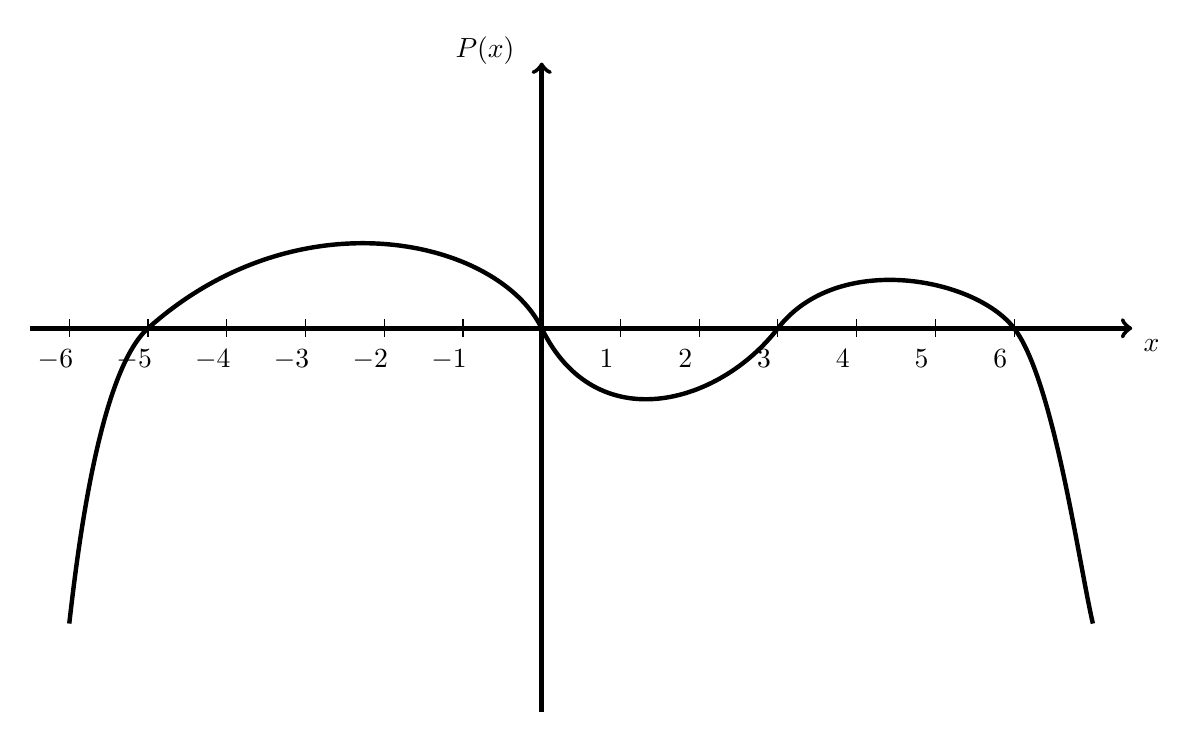
\begin{tikzpicture}[y=0.75cm, x=1.0cm,font=\sffamily]
      \begin{scope}[shift={(0,0)}]
        % axis
        \draw[ultra thick,->] (-6.5,0) -- coordinate (x axis mid) (7.5,0)
            node[anchor = north west] {$x$}; 
        \draw[ultra thick,->] (0,-6.5) -- coordinate (y axis mid) (0,4.5) 
            node[anchor = east,shift={(-0.2,0.2)}]  {$P(x)$};

      \draw[ultra thick,black]
       (-6, -5) .. controls +( 85:1)   and +(230:1)    .. (-5, 0)
       (-5,  0) .. controls +( 50:3)   and +(110: 1.6) .. ( 0, 0)
       ( 0,  0) .. controls +(290:2.0) and +(240: 1.5) .. ( 3, 0)
       ( 3,  0) .. controls +( 60:1.5) and +(120: 1.0) .. ( 6, 0)
       ( 6,  0) .. controls +(300:1)   and +(100: 1)   .. ( 7,-5)
       ;

       \foreach \x in {-6,-5,...,-1,1,2,...,6} {
          \draw (\x,0.15) -- (\x,-0.15) node[yshift=-1,xshift=-5,anchor=north] {$\x$};
        }


    \end{scope}

    \end{tikzpicture}


  \vfill
\end{problem}


\actTitle{Factoring Polynomials}
\begin{problem}
\item For each function below express the result as a polynomial plus
  a remainder.
  \begin{subproblem}
  \item ${\displaystyle \frac{8x^4+17x^3-14x-8}{x+2} }$.
    \vfill
  \item ${\displaystyle \frac{x^4-1}{x+1} }$.
    \vfill
  \item ${\displaystyle \frac{x^4-1}{x^2+4} }$.
    \vfill
  \end{subproblem}

  \clearpage
  
\item Make a rough sketch of the polynomial
  \begin{eqnarray*}
    h(x) & = & -2x^3+4x^2+10x-12
  \end{eqnarray*}

  \begin{tikzpicture}[y=0.9cm, x=0.9cm,font=\sffamily]
    % bounds
    \def\lowX{-5.5}
    \pgfmathtruncatemacro\startX{round(0.5+\lowX)}
    \pgfmathsetmacro\nextXValue{int(\startX+1)}
    \def\highX{5.5}
    \def\lowY{-5.5}
    \def\highY{5.5}
    \pgfmathsetmacro\nextYValue{int(\lowY+1)}
    % ticks
    \draw[step = 1, gray, very thin,dashed,opacity=0.85] (\lowX, \lowY) grid ( \highX,\highY);
    % axis
    \draw[thick,->] (\lowX,0) -- coordinate (x axis mid) (\highX,0) node[anchor = north west] {$x$};
    \draw[thick,->] (0,\lowY) -- coordinate (y axis mid) (0,\highY) node[anchor = south east] {$y$};
    \foreach \y in {-5,-4,...,-1,1,2,...,\highY} {
      \draw (1pt, \y) -- (-1pt, \y) node[yshift=-6,xshift=-1,anchor=east] {$\y$};
    }
    \foreach \x in {-5,-4,...,-1,1,2,...,\highX} {
      \draw (\x,1pt) -- (\x,-1pt) node[yshift=-5,xshift=-1,anchor=east] {$\x$};
    }
    %\draw (0,6.0) node [anchor=south] {Comparing Shifted Functions};
  \end{tikzpicture}

  \vfill

  \clearpage

\item Given the graph of a polynomial below, determine the smallest
  possible degree of the polynomial.


  \clearpage

\item 
  \begin{subproblem}
  \item 
    \vfill
  \item 
    \vfill
  \end{subproblem}

\end{problem}

\postClass

\begin{problem}
\item Briefly state two ideas from today's class.
  \begin{itemize}
  \item 
  \item 
  \end{itemize}
\item 
  \begin{subproblem}
    \item
  \end{subproblem}
\end{problem}


%%% Local Variables:
%%% mode: latex
%%% TeX-master: "../labManual"
%%% End:

